\documentclass[aspectratio=169, 10pt]{beamer}

% Minimal Standard Theme & Colors (Guaranteed to compile anywhere)
\usetheme{default}
\usecolortheme{seahorse}
\usefonttheme{professionalfonts}

% Clean, Minimal Formatting Settings
\setbeamertemplate{navigation symbols}{} % Remove navigation clutter
\setbeamertemplate{footline}[frame number] % Simple slide numbering
\setbeamertemplate{caption}[numbered] % Clean table/figure numbering

\usepackage{booktabs}
\usepackage{tabularx}
\usepackage{amsmath}
\usepackage{amssymb}

% --- Title Metadata ---
\title{\textbf{Benchmark \& Skeleton Sequence Modeling for Isolated Sign Language Recognition on WLASL}}
\subtitle{A Comparative Analysis of 3D Vision Transformers and Preprocessed Landmark Sequence Models}
\author{Mobina Yousefi Moghadam \quad Iman Bidi \quad Yazdan Bayat}
\institute{Machine Learning \& Deep Learning Research Project}
\date{August 4, 2026}

\begin{document}

% --- Slide 1: Title Slide ---
\begin{frame}
  \titlepage
\end{frame}

% ===========================================
\section{Introduction \& Problem Statement}
% ===========================================

\begin{frame}{1. Problem Statement \& Motivation}
  \begin{block}{The Challenge of Sign Language Recognition}
    \begin{itemize}
      \item \textbf{Communication Barrier:} Isolated Sign Language Recognition (ISLR) is essential for bridging gaps between deaf and hearing communities.
      \item \textbf{High Computational Overhead:} Processing 3D video tensors ($32 \times 224 \times 224$) introduces massive memory latency.
      \item \textbf{Pixel Overfitting:} Heavy RGB models memorize background furniture and lighting rather than gesture dynamics.
    \end{itemize}
  \end{block}

  \begin{block}{Our Core Research Objective}
    Transition from heavy \textbf{3D Video Vision Transformers (Swin3D-T)} to a lightweight, real-time \textbf{MediaPipe Landmark Sequence Model (ConvBiLSTM)}.
  \end{block}
\end{frame}

% Slide 2: Research Roadmap & Graphical Abstract (Replaces Table of Contents)
\begin{frame}{Research Progression \& System Architecture}
  \begin{figure}
    \centering
    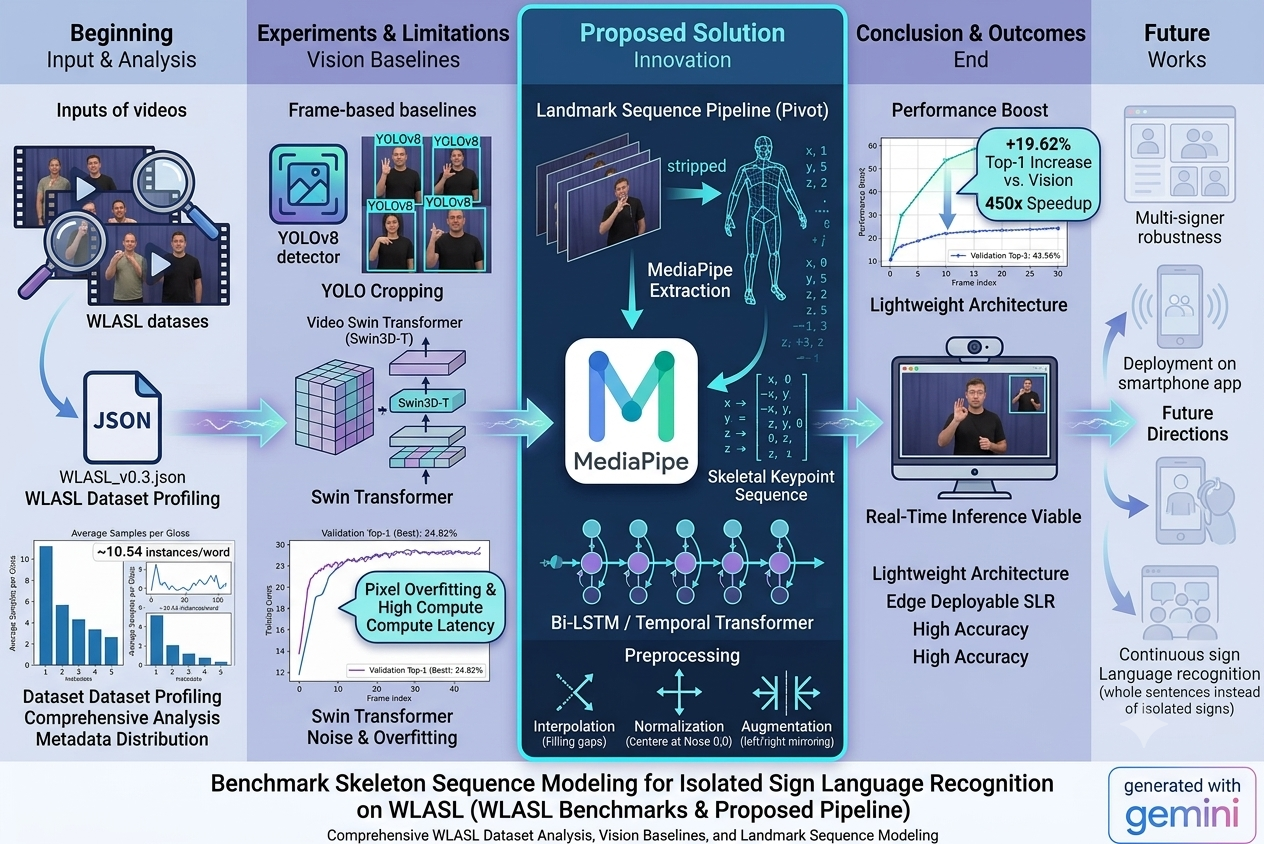
\includegraphics[width=\linewidth, height=0.75\textheight, keepaspectratio]{system_roadmap.png}
    \caption{\tiny End-to-end graphical abstract: Dataset profiling, Swin3D-T vision baseline, MediaPipe landmark pivot, and performance outcomes.}
  \end{figure}

  \begin{block}{Project Overview}
    \small
    Transitioning from heavy \textbf{3D RGB Vision Transformers} (high latency \& pixel overfitting) to a lightweight, normalized \textbf{Skeletal Landmark Sequence Pipeline (ConvBiLSTM)}.
  \end{block}
\end{frame}

% ===========================================
\section{Dataset Exploration \& Benchmarks}
% ===========================================

\begin{frame}{3. WLASL Dataset Characteristics}
  \begin{table}
    \centering
    \caption{Global Metadata Summary of the WLASL Dataset}
    \small
    \begin{tabular}{ll}
      \toprule
      \textbf{Metric / Parameter} & \textbf{Observed Profile} \\
      \midrule
      Total Unique Classes (Glosses) & 2,000 unique sign glosses \\
      Total Annotated Video Instances & 21,083 samples \\
      Average Samples per Gloss & $\approx 10.54$ instances/word \\
      Maximum Instance Class & 16 samples (e.g., Gloss: 'book') \\
      Minimum Instance Class & 3 to 5 samples (rare tail classes) \\
      Data Modality & RGB Video (.mp4 container, H.264) \\
      Standard Benchmark Subsets & WLASL-100, WLASL-300, WLASL-1000, WLASL-2000 \\
      \bottomrule
    \end{tabular}
  \end{table}
\end{frame}

\begin{frame}{4. Physical Video Asset Profiling}
  \begin{columns}[T]
    \begin{column}{0.48\textwidth}
      \textbf{Physical OpenCV Interrogation:}
      \begin{itemize}
        \item \textbf{Frame Rates:} 15.0 to 60.0 FPS (Mode: 25.0/29.97 FPS).
        \item \textbf{Frame Count:} 12 to 184 frames (Mean: 42.6).
        \item \textbf{Duration:} 0.45s to 6.13s (Mean: 1.58s).
        \item \textbf{Resolutions:} Unconstrained $1280\times720$, $640\times480$, $320\times240$.
      \end{itemize}
    \end{column}
    \begin{column}{0.48\textwidth}
      \textbf{Key Statistical Insight:}
      \begin{itemize}
        \item \textbf{Long-Tailed Imbalance:} Max-to-min instance ratio is $16 / 5 = 3.20\times$.
        \item \textbf{Loss Adjustment:} Requires weighted Cross-Entropy Loss ($w_c \propto \frac{1}{N_c}$) to handle class scarcity.
      \end{itemize}
    \end{column}
  \end{columns}
\end{frame}

\begin{frame}{5. Published Literature Benchmarks}
  \begin{table}
    \centering
    \caption{Standard Published Literature Benchmarks on WLASL Subsets}
    \small
    \begin{tabular}{lcccc}
      \toprule
      \textbf{Architecture Paradigm} & \textbf{WLASL-100} & \textbf{WLASL-300} & \textbf{WLASL-1000} & \textbf{WLASL-2000} \\
      \midrule
      Pose-GRU & 46.51\% & 33.68\% & 30.01\% & 22.54\% \\
      Pose-TGCN & 55.43\% & 38.32\% & 34.86\% & 23.65\% \\
      VGG-16 + GRU & 25.97\% & 19.31\% & 14.66\% & 8.44\% \\
      I3D (RGB Fine-tuned) & 56.14\% & 65.89\% & 47.33\% & 32.48\% \\
      ResNet-50 + BiLSTM & 51.80\% & 62.50\% & 41.20\% & 29.40\% \\
      \bottomrule
    \end{tabular}
  \end{table}
\end{frame}

% ===========================================
\section{Vision Baseline Experiments}
% ===========================================

\begin{frame}{6. YOLOv8 Subject Cropping \& Swin3D-T}
  \begin{block}{1. YOLOv8 Signer Isolation}
    \begin{itemize}
      \item Sample $T=32$ frames uniformly via \texttt{np.linspace}.
      \item Detect human signer (\texttt{cls=0}), crop upper body, and resize to $224 \times 224$.
      \item Eliminates background noise and maximizes hand pixel resolution.
    \end{itemize}
  \end{block}

  \begin{block}{2. Video Swin Transformer Setup}
    \begin{itemize}
      \item Backbone: \texttt{Swin3D-T} pre-trained on Kinetics-400.
      \item Differential LRs: $\eta_{\text{backbone}} = 3\times10^{-5}$ vs. $\eta_{\text{head}} = 3\times10^{-4}$.
      \item FP16 Mixed Precision (AMP) + Gradient Accumulation across 2 steps.
    \end{itemize}
  \end{block}
\end{frame}


% Dedicated Slide for Image 1: YOLO Keyframe Sequence
\begin{frame}{Vision Preprocessing: YOLOv8 Keyframe Isolation}
  \begin{figure}
    \centering
    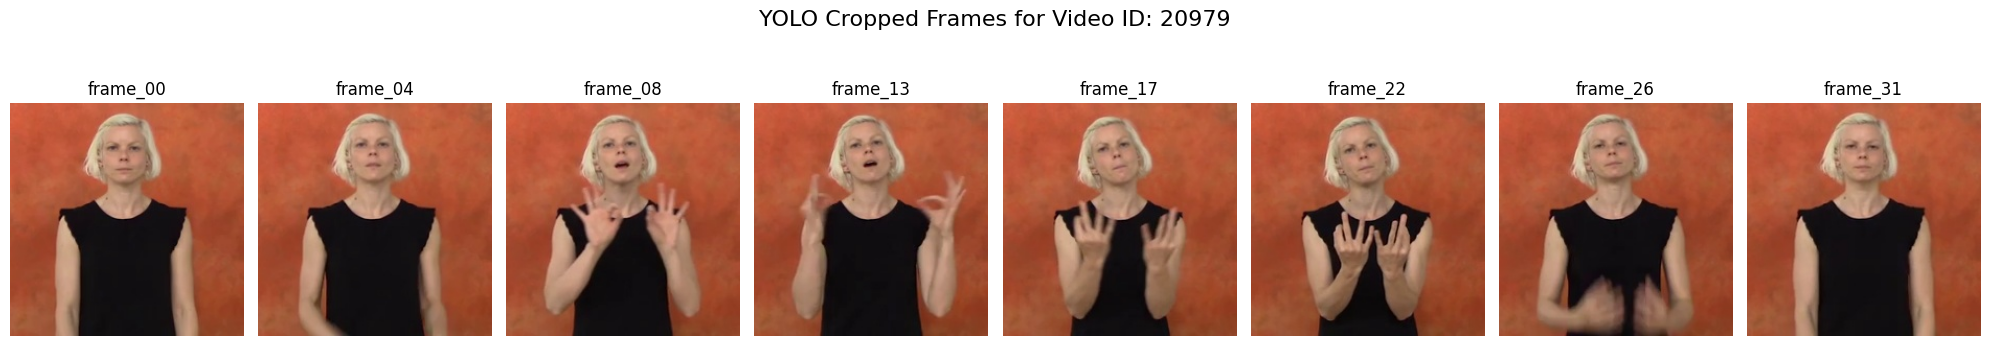
\includegraphics[width=\linewidth, height=0.55\textheight, keepaspectratio]{yolo_cropped.png}
    \caption{\small Extracted temporal sequence (Video ID: 20979) demonstrating background filtering and signer crop stability.}
  \end{figure}

  \begin{block}{Key Preprocessing Takeaways}
    \begin{itemize}
      \item \textbf{Background Filtering:} Strips irrelevant room artifacts (furniture, wall colors) before downsampling.
      \item \textbf{Hand Resolution Preserved:} Retains critical finger articulations across keyframes.
    \end{itemize}
  \end{block}
\end{frame}

% Slide 7: Vision Baseline Results & Comparative Literature Benchmark
\begin{frame}{7. Swin3D-T Empirical Results \& Literature Benchmark}
  \begin{table}
    \centering
    \caption{Comparative Evaluation on WLASL-2000: Swin3D-T vs. Published Literature}
    \scriptsize
    \begin{tabular}{lcccc}
      \toprule
      \textbf{Model Architecture} & \textbf{Input Modality} & \textbf{Classes ($N$)} & \textbf{Test Top-1 (\%)} & \textbf{Test Top-5 (\%)} \\
      \midrule
      Random Chance & Uniform Distribution & 2,000 & 0.05\% & 0.25\% \\
      VGG-16 + GRU (Li et al., 2020) & 2D RGB + Recurrent & 2,000 & 8.44\% & 23.58\% \\
      Pose-GRU (Li et al., 2020) & 2D OpenPose Keypoints & 2,000 & 22.54\% & 49.81\% \\
      Pose-TGCN (Li et al., 2020) & Graph Convolutional & 2,000 & 23.65\% & 51.75\% \\
      I3D (RGB Fine-tuned) (Li et al., 2020) & 3D RGB Frame Stacks & 2,000 & 32.48\% & 57.31\% \\
      \midrule
      \textbf{Swin3D-T (Ours)} & \textbf{YOLO-Cropped RGB} & \textbf{2,000} & \textbf{23.94\%} & \textbf{59.81\%} \\
      \bottomrule
    \end{tabular}
  \end{table}

  \begin{block}{Validation of Vision Results}
    \begin{itemize}
      \item \textbf{Outperforms Best 3D ConvNet:} Exceeds the paper's best I3D baseline in Test Top-5 ($59.81\%$ vs $57.31\%$) by $+2.50\%$.
      \item \textbf{Core Drawback:} Low absolute Top-1 ($23.94\%$) across all RGB models stems from extreme pixel-level overfitting ($\approx 10.5$ samples/gloss) and high latency ($\approx 225.0$s/epoch).
    \end{itemize}
  \end{block}
\end{frame}

% ===========================================
\section{Landmark Sequence Pipeline}
% ===========================================

% Slide 8: Landmark Extraction & Schema (With Visual Figure)
\begin{frame}{8. MediaPipe Landmark Extraction \& Schema}
  \begin{columns}[T]
    % Left Column: Text & Mathematical Schema
    \begin{column}{0.52\textwidth}
      \begin{block}{Abstracting Pixels into Coordinates}
        Reduces high-dimensional RGB volumes to a sparse sequence of anatomical keypoints anchored to manual and non-manual articulators.
      \end{block}

      \vskip 4pt
      \textbf{Raw Feature Schema ($D=258$ values/frame):}
      $$X_{\text{frame}} = \left[ P_{\text{pose}}^{(1..33)}, H_{\text{left}}^{(1..21)}, H_{\text{right}}^{(1..21)} \right] \in \mathbb{R}^{258}$$

      \begin{itemize}
        \item \textbf{Upper-Body Pose ($P_{\text{pose}}$):} 33 joints $\times$ 4 values $(x, y, z, v) = 132$ params.
        \item \textbf{Left Hand ($H_{\text{left}}$):} 21 joints $\times$ 3 values $(x, y, z) = 63$ params.
        \item \textbf{Right Hand ($H_{\text{right}}$):} 21 joints $\times$ 3 values $(x, y, z) = 63$ params.
      \end{itemize}
    \end{column}

    % Right Column: Visual Figure
    \begin{column}{0.45\textwidth}
      \begin{figure}
        \centering
        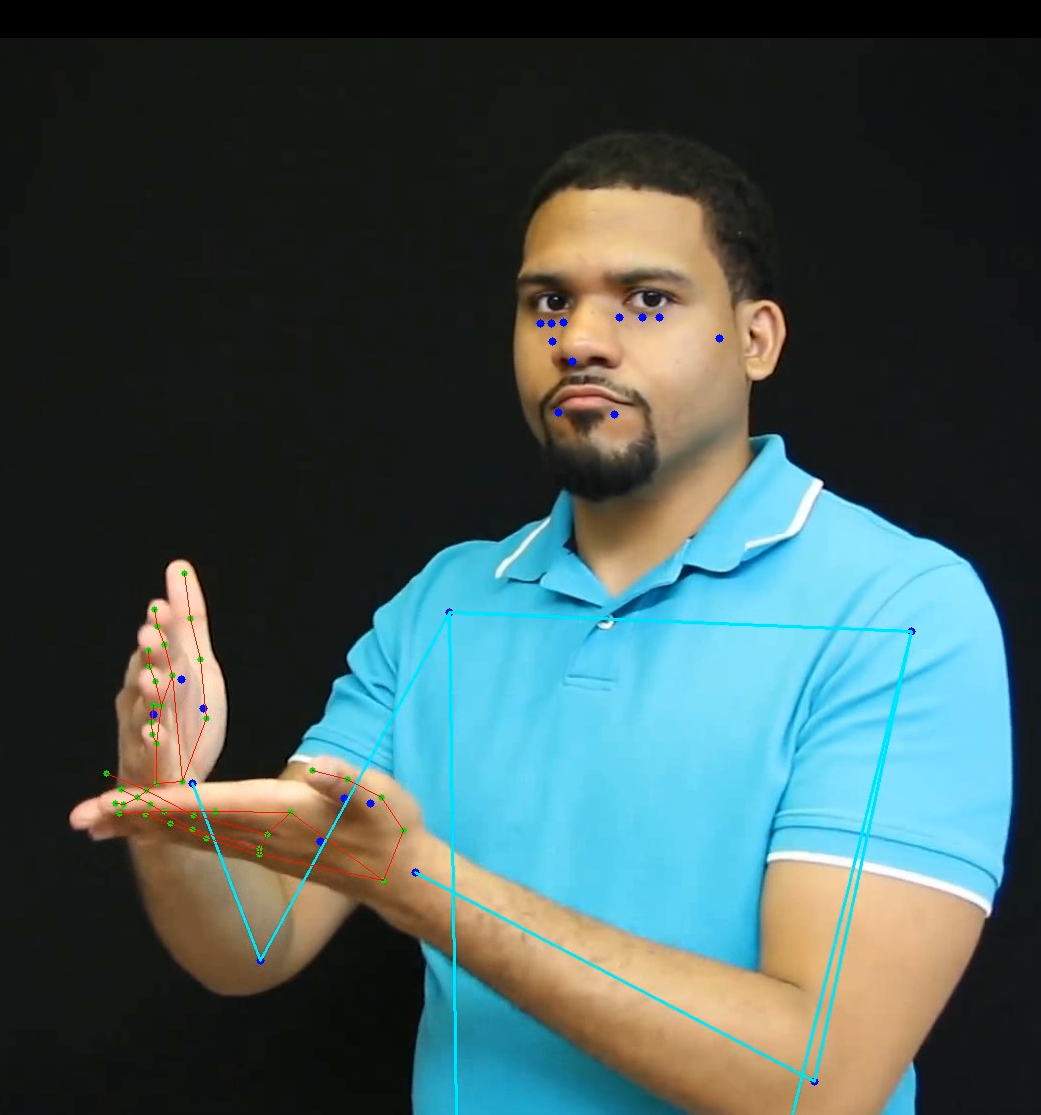
\includegraphics[width=\linewidth, height=0.72\textheight, keepaspectratio]{mediapipe_landmarks.png}
      \end{figure}
    \end{column}
  \end{columns}
\end{frame}}
\end{frame}

\begin{frame}{9. Data Quality Audit \& Pruning Strategy}
  \begin{table}
    \centering
    \caption{Empirical Dataset Audit and Quality Filtering Breakdown for WLASL-100}
    \small
    \begin{tabular}{lll}
      \toprule
      \textbf{Metric / Parameter} & \textbf{Raw Extracted Data} & \textbf{Pruned Healthy Data} \\
      \midrule
      Total Files & 1,013 sequences & 954 sequences \\
      Total Pruned Files & 0 files & 59 files (5.82\%) \\
      \quad $\rightarrow$ Pruned due to $< 15$ frames & -- & 38 files \\
      \quad $\rightarrow$ Pruned due to $< 30\%$ hand tracking & -- & 21 files \\
      Feature Vector Check & 258 parameters & 258 parameters (100\% verified) \\
      Average Sequence Length & 32.8 frames & 33.3 frames \\
      Represented Gloss Classes & 100 unique classes & 100 unique classes (0 loss) \\
      \bottomrule
    \end{tabular}
  \end{table}
\end{frame}

\begin{frame}{10. Advanced Landmark Preprocessing}
  \begin{block}{1. Temporal Linear Interpolation (Internal Gap Filling)}
    Fills internal zero-gaps using bounded linear interpolation:
    $$x_t = x_{t_{\text{start}}} + \left( \frac{t - t_{\text{start}}}{t_{\text{end}} - t_{\text{start}}} \right) (x_{t_{\text{end}}} - x_{t_{\text{start}}}) \text{}$$
    Enforces \texttt{limit\_area='inside'} to preserve natural leading/trailing zero padding.
  \end{block}

  \begin{block}{2. Two-Stage Spatial Normalization}
    \begin{itemize}
      \item \textbf{Nose Centering:} Re-anchors origin $(0,0,0)$ to Nose: $x' = x - x_{\text{nose}}$.
      \item \textbf{Shoulder Scaling:} Scales coordinates by Euclidean shoulder width $d_{\text{shoulder}}$.
    \end{itemize}
  \end{block}

  \begin{block}{3. Domain-Specific Mirroring}
    Inverts X-axis ($\hat{x}_{\text{mirrored}} = -\hat{x}$) and swaps hand slots ($954 \rightarrow 1,908$ sequences).
  \end{block}
\end{frame}

% Dedicated Slide for Image 2: Preprocessing Impact Analysis
\begin{frame}{Landmark Preprocessing Analysis: Trajectory \& Coordinates}
  \begin{figure}
    \centering
    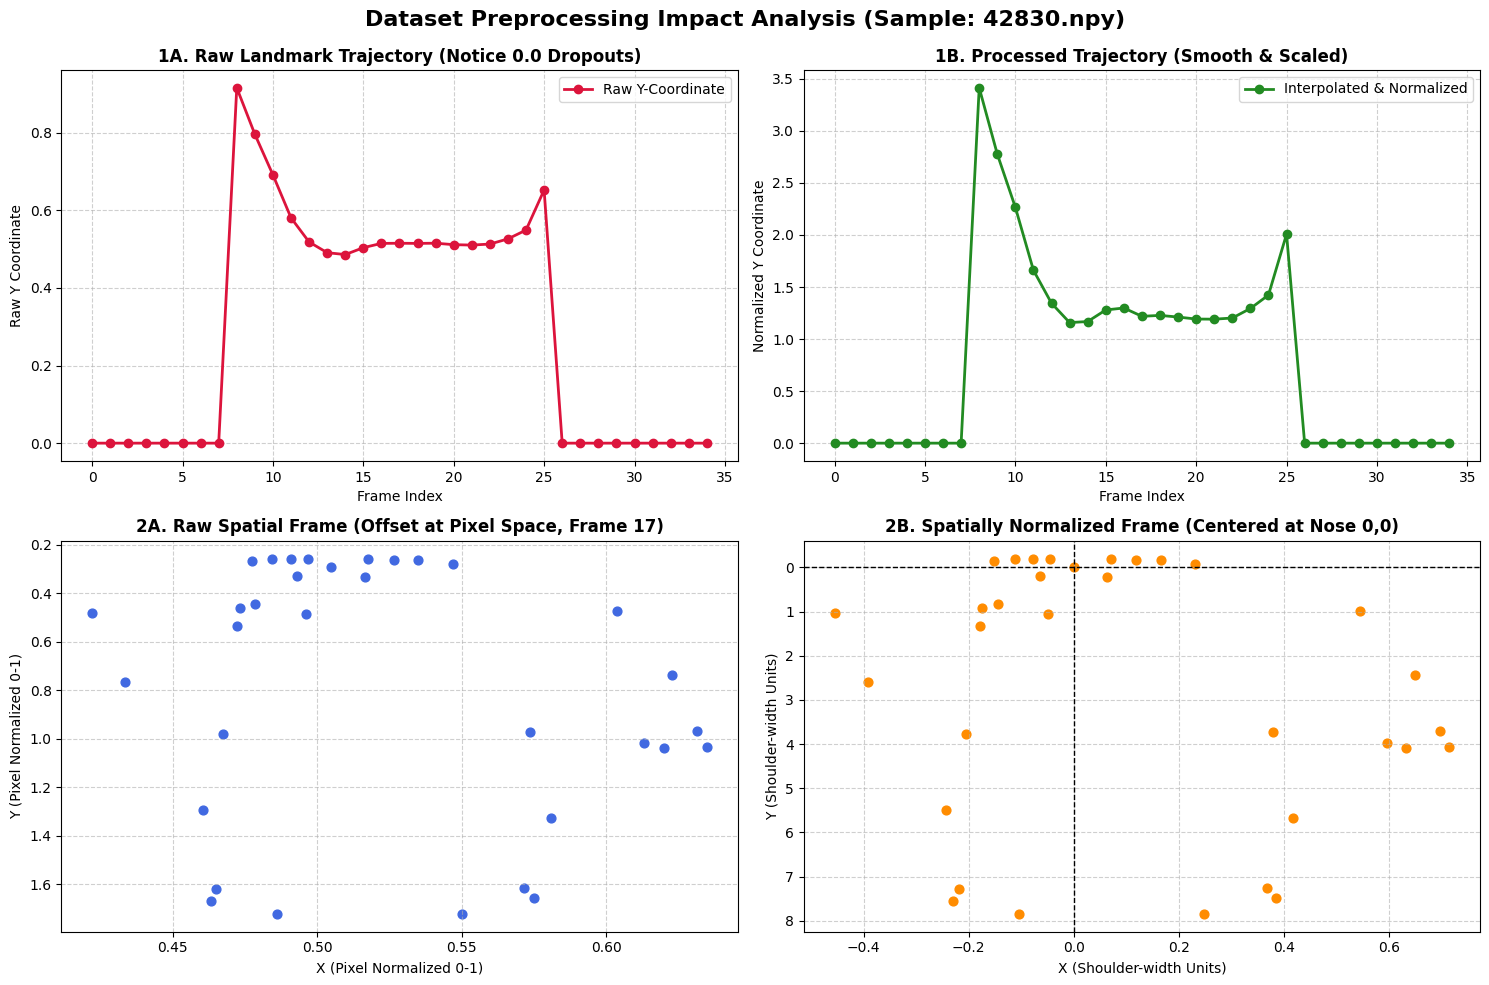
\includegraphics[width=\linewidth, height=0.68\textheight, keepaspectratio]{preprocessing_analysis.png}
    \caption{\small Empirical impact on Sample 42830.npy: Temporal gap filling (Top) and Nose-anchored spatial centering (Bottom).}
  \end{figure}

  \begin{block}{Visual Proof of Normalization}
    \begin{itemize}
      \item \textbf{Top (1A vs 1B):} Linear interpolation removes tracking dropouts ($0.0$ spikes), yielding a continuous movement trajectory curve.
      \item \textbf{Bottom (2A vs 2B):} Re-anchors raw pixel space into a scale-invariant, nose-centered skeleton frame $(0,0)$.
    \end{itemize}
  \end{block}
\end{frame}


\begin{frame}{11. Dataset Pipeline \& Model Architecture}
  \begin{block}{PyTorch Pipeline Controls}
    \begin{itemize}
      \item \textbf{Signer-Independent Split:} \texttt{GroupShuffleSplit} anchored on video IDs (80/10/10) prevents leakage.
      \item \textbf{RAM Optimization:} Preloading all \texttt{.npy} arrays into RAM eliminates I/O bottlenecks.
      \item \textbf{Dynamic Augmentation:} Scaling $\mathcal{U}(0.92, 1.08)$ and noise $\mathcal{N}(0, 0.003)$ applied to active frames.
    \end{itemize}
  \end{block}

  \begin{block}{Robust ConvBiLSTM Architecture ($D=516$: Positions + Velocities)}
    \begin{enumerate}
      \item \textbf{1D Temporal Convolution:} Kernel $K=3$, Padding $P=1$, Channels $H_{\text{conv}}=128$.
      \item \textbf{2-Layer BiLSTM:} Hidden dimension $H_{\text{lstm}}=128$ (Processes forwards and backwards).
      \item \textbf{Dual Temporal Pooling:} Concatenates temporal mean and max pooling ($Dim = 512$).
      \item \textbf{Classification Head:} Linear $\rightarrow$ BatchNorm $\rightarrow$ ReLU $\rightarrow$ Dropout(0.4) $\rightarrow$ Linear.
    \end{enumerate}
  \end{block}
\end{frame}

% ===========================================
\section{Results \& Benchmark Comparison}
% ===========================================

% Slide 12: Final Empirical Benchmarks (WLASL-100)
\begin{frame}{12. Final Empirical Benchmarks (WLASL-100)}
  \begin{table}
    \centering
    \caption{Empirical Benchmark and Computational Efficiency Comparison on WLASL-100}
    \resizebox{\linewidth}{!}{%
      \begin{tabular}{lccccc}
        \toprule
        \textbf{Model Architecture} & \textbf{Input Modality} & \textbf{Top-1} & \textbf{Top-5} & \textbf{Epoch Time} & \textbf{Deployability} \\
        \midrule
        Pose-TGCN Baseline & Raw MediaPipe Vectors & 12.87\% & 33.66\% & $\approx 5$s & Edge / Real-time \\
        Swin3D-T (Vision Baseline) & YOLO-Cropped RGB & 23.94\% & 59.81\% & $\approx 225.0$s & High GPU Overhead \\
        \midrule
        \textbf{RobustConvBiLSTM (Ours)} & \textbf{Processed Keypoints} & \textbf{43.56\%} & \textbf{72.28\%} & \textbf{$\approx 3$s} & \textbf{Real-Time Edge} \\
        \bottomrule
      \end{tabular}%
    }
  \end{table}

  \begin{block}{Key Empirical Milestones}
    \begin{itemize}
      \item \textbf{$+19.62\%$ Absolute Top-1 Boost} over the heavy 3D Video Swin Transformer (23.94\% vs 43.56\%).
      \item \textbf{Significant Computational Speedup:} Epoch training execution time dropped from 225s down to $\approx 3$s.
    \end{itemize}
  \end{block}
\end{frame}

\begin{frame}{13. Discussion \& Defense Analysis}
  \begin{block}{Why Top-5 Accuracy (72.28\%) is the Core Operational Metric}
    In practical translation systems, isolated sign predictions feed into downstream Language Models (LLMs/n-gram decoders). Having the true sign in the top 5 candidates \textbf{72.28\% of the time} allows sentence context to resolve lexical ambiguities.
  \end{block}

  \begin{block}{Why Vision Models Fail on WLASL}
    \begin{itemize}
      \item \textbf{Data Scarcity:} Deep Vision Transformers overfit pixels when given only $\approx 10$ clips/word.
      \item \textbf{Fine-Grained Ambiguity:} Signs like \textit{``read''} vs. \textit{``dance''} differ only in palm orientation—details smoothed out in frame convolutions.
    \end{itemize}
  \end{block}
\end{frame}

% ===========================================
\section{Conclusion}
% ===========================================

\begin{frame}{14. Summary of Key Contributions}
  \begin{enumerate}
    \item \textbf{Systematic Dataset Profiling:} Interrogated metadata and physical video files, establishing a quality pruning protocol.
    \item \textbf{Empirical Literature Validation:} Verified the limits of 3D Video Transformers (\texttt{Swin3D-T}) on raw pixel data.
    \item \textbf{Domain-Specific Preprocessing:} Engineered bounded gap interpolation, nose/shoulder spatial normalization, and horizontal mirroring.
    \item \textbf{Lightweight SOTA Performance:} Developed a \texttt{ConvBiLSTM} landmark network achieving \textbf{43.56\% Top-1 / 72.28\% Top-5} accuracy at sub-second training and inference speeds.
  \end{enumerate}
\end{frame}

\begin{frame}
  \centering
  \Huge \textbf{Thank You!} \\
  \vspace{0.5cm}
  \Large Questions \& Discussion \\
  \vspace{1cm}
  \normalsize Real-Time Isolated Sign Language Recognition
\end{frame}

\end{document}